\documentclass[11pt,a4paper]{article}

% ---------------------------------------------------------------
% Packages
% ---------------------------------------------------------------
\usepackage[T1]{fontenc}
\usepackage{amsmath, amsthm, mathtools}
\usepackage{libertinus}
\usepackage{libertinust1math}
\usepackage{bm}
\usepackage{graphicx}
\usepackage{xcolor}
\usepackage{tikz}
\usetikzlibrary{arrows.meta}
\usepackage[most]{tcolorbox}
\usepackage{booktabs}
\usepackage{tabularx}
\usepackage[numbers,sort&compress]{natbib}
\usepackage{microtype}
\usepackage{parskip}
\usepackage[margin=2.5cm, headheight=20pt]{geometry}
\usepackage{titlesec}
\usepackage{fancyhdr}
\usepackage{lastpage}
\usepackage{hyperref}
\usepackage[capitalise,noabbrev]{cleveref}

\numberwithin{equation}{section}

% ---------------------------------------------------------------
% Corporate colours (sampled from the FAU logo) and layout
% ---------------------------------------------------------------
\definecolor{faublue}{RGB}{0,47,108}
\definecolor{fautech}{RGB}{119,159,181}

\hypersetup{colorlinks=true, linkcolor=faublue, citecolor=faublue, urlcolor=faublue,
  pdftitle={Stationary Diffusion in Two Dimensions}, pdfauthor={Ali Ghelichkhani}}

\titleformat{\section}{\sffamily\Large\bfseries\color{faublue}}{\thesection}{0.75em}{}
\titleformat{\subsection}{\sffamily\large\bfseries\color{faublue}}{\thesubsection}{0.7em}{}
\titleformat{\paragraph}[runin]{\sffamily\bfseries\color{faublue}}{}{0pt}{}
\titlespacing*{\paragraph}{0pt}{1.2ex plus 0.4ex}{0.6em}

\pagestyle{fancy}
\fancyhf{}
\fancyhead[L]{\sffamily\small\color{fautech}Materials Simulation Practical~1 \textbullet{} Part~I}
\fancyhead[R]{\raisebox{-0.2\height}{
\includegraphics[height=0.42cm]{figures/ww8.png}}}
\fancyfoot[L]{\sffamily\small\color{fautech}A.~Ghelichkhani}
\fancyfoot[R]{\sffamily\small\color{fautech}\thepage\ / \pageref*{LastPage}}
\renewcommand{\headrule}{\hbox to\headwidth{\color{fautech}\leaders\hrule height 0.4pt\hfill}}

% Task statements of the tutorial script (paraphrased); the box never separates from the
% heading above it, because "before" allows no page break
\newtcolorbox{task}[1]{enhanced, sharp corners, frame hidden,
  colback=fautech!12, borderline west={2.5pt}{0pt}{faublue},
  left=9pt, right=9pt, top=6pt, bottom=6pt, after skip=12pt,
  before={\par\nopagebreak\vskip 6pt},
  fontupper=\sffamily\small,
  before upper={{\bfseries\color{faublue}Task~#1.}\enspace}}
\setcounter{MaxMatrixCols}{20}

\theoremstyle{definition}
\newtheorem{assumption}{Assumption}
\theoremstyle{remark}
\newtheorem{remark}{Remark}[section]

% ---------------------------------------------------------------
% Notation
% ---------------------------------------------------------------
\newcommand{\R}{\mathbb{R}}
\newcommand{\grad}{\nabla}
\newcommand{\bigO}[1]{\mathcal{O}\!\left(#1\right)}
\newcommand{\bj}{\bm{j}}
\newcommand{\bn}{\bm{n}}
\newcommand{\be}{\bm{e}}
\newcommand{\bD}{\mathbf{D}}
\newcommand{\bQ}{\mathbf{Q}}
\newcommand{\bA}{\mathbf{A}}
\newcommand{\bT}{\mathbf{T}}
\newcommand{\bI}{\mathbf{I}}
\newcommand{\bW}{\mathbf{W}}
\newcommand{\bS}{\mathbf{S}}
\newcommand{\bLambda}{\bm{\Lambda}}
\newcommand{\brho}{\bm{\rho}}
\newcommand{\bb}{\bm{b}}
\newcommand{\rhoUpper}{\bar{\rho}_{\mathrm{upper}}}
\newcommand{\rhoLower}{\bar{\rho}_{\mathrm{lower}}}
\newcommand{\jleft}{\bar{j}_{\mathrm{left}}}
\newcommand{\jright}{\bar{j}_{\mathrm{right}}}

\definecolor{cdiag}{RGB}{0,0,0}
\definecolor{cx}{RGB}{0,114,178}
\definecolor{cy}{RGB}{213,94,0}
\definecolor{cdir}{RGB}{0,114,178}
\definecolor{cneu}{RGB}{213,94,0}

\begin{document}

% ===============================================================
% Title page
% ===============================================================
\begin{titlepage}
  \noindent
  
\includegraphics[height=2.0cm]{figures/fau-techfak.png}\hfill
  \raisebox{0.6cm}{
\includegraphics[height=1.1cm]{figures/ww8.png}}

  \vspace{0.2cm}
  {\color{fautech}\rule{\textwidth}{0.6pt}}\\[0.1cm]
  {\sffamily\small\color{fautech}Institute of Materials Simulation (WW8)\hfill
    Winter semester 2026/27}

  \vspace*{3.4cm}
  {\sffamily\large\color{fautech}\textls[120]{MATERIALS SIMULATION PRACTICAL 1}\par}
  \vspace{0.5cm}
  {\sffamily\bfseries\color{faublue}\fontsize{30}{36}\selectfont
    Stationary Diffusion\\[0.1em] in Two Dimensions\par}
  \vspace{0.5cm}
  {\sffamily\Large\color{faublue}Governing Equations and Finite-Difference Discretization\par}
  \vspace{0.7cm}
  {\color{faublue}\rule{3cm}{2pt}}\par
  \vspace{0.4cm}
  {\sffamily\large Report, Part~I \textbullet{} Tasks~1 to~4\par}

  \vfill
  {\sffamily
  \renewcommand{\arraystretch}{1.35}
  \begin{tabular}{@{}>{\small\color{fautech}}l@{\hspace{1.2em}}l@{}}
    Author     & Ali Ghelichkhani \\
    E-mail     & \href{mailto:ali.ghelichkhani@fau.de}{ali.ghelichkhani@fau.de} \\
    Supervisor & Xingchen Tan \\
    Module     & Foundations of Materials Simulation \\
    Institute  & Institute of Materials Simulation (WW8), FAU Erlangen-N\"urnberg \\
    Part~II    & Task~5, Jupyter notebook \texttt{task5\_fd\_solver.ipynb} \\
    Date       & \today
  \end{tabular}\par}
\end{titlepage}

% ===============================================================
% Abstract and contents
% ===============================================================
\section*{Abstract}
  We derive the partial differential equation that governs diffusion of a single species
  in a two-dimensional anisotropic medium and prepare it for numerical solution by finite
  differences. Combining Fick's first law with the continuity equation yields Fick's
  second law, a parabolic equation whose stationary limit is elliptic. In the principal
  axes of the diffusion tensor, the stationary equation reduces to
  $\partial^2_{xx}\rho + P\,\partial^2_{yy}\rho = 0$, where $P$ is the ratio of the two
  principal diffusivities, and a rescaling of one coordinate transforms it into the
  Laplace equation. We discretize the equation with a second-order central-difference
  scheme on an equidistant mesh, introduce a row-wise node numbering, and incorporate
  Dirichlet conditions by elimination and Neumann conditions by ghost nodes that preserve
  second-order accuracy. The resulting linear system is sparse, pentadiagonal, block
  tridiagonal and irreducibly diagonally dominant; it is a nonsingular M-matrix whose
  only asymmetry stems from the Neumann rows and is removed by a diagonal scaling. These
  properties guarantee a unique discrete solution that is non-negative for physically
  admissible data and depends monotonically on them, and they prepare the implementation
  reported in Part~II.

\tableofcontents
\clearpage

% ===============================================================
\section{Introduction}\label{sec:intro}
% ===============================================================

Diffusion is the net transport of matter that results from the random thermal motion of
individual particles. Where the concentration of a species varies in space, more
particles statistically jump from regions of high concentration into regions of low
concentration than in the opposite direction, so that an initially inhomogeneous material
homogenizes over time. Diffusion controls many processes in materials science, among them
homogenization annealing, precipitation, oxidation and the motion of adsorbed atoms on
surfaces. On the continuum scale it is described phenomenologically by Fick's two laws of
diffusion~\citep{fick1855, crank1975}, which relate the diffusion flux to the
concentration gradient and express the conservation of mass.

In this report we treat a two-dimensional domain on which a single species diffuses, for
example adatoms on a crystal surface. We denote by $\rho(x,y)$ the concentration of the
diffusing species, by $\bj(x,y)$ the diffusion flux and by $\bD$ the symmetric tensor of
diffusion coefficients that connects the flux to the concentration gradient. Following the
tutorial script~\citep{script}, we derive and classify the governing equation
(\cref{sec:pde}), discretize it by finite differences (\cref{sec:fd}), incorporate
boundary conditions (\cref{sec:bc}) and assemble and analyse the resulting linear system
(\cref{sec:system}). Stationary heat conduction obeys an equation of identical structure,
with temperature in place of concentration and the thermal conductivity tensor in place of
$\bD$, so all results apply to it as well. The numerical implementation and its
verification (Task~5) form Part~II and are provided as a Jupyter notebook. Each task of
the script is restated, in paraphrased form, in a shaded box at the beginning of the
section that answers it, and \cref{tab:taskmap} gives an overview.

\begin{table}[ht]
  \centering
  \caption{Correspondence between the tasks of the tutorial script and this report.}
  \label{tab:taskmap}
  \begin{tabularx}{0.85\linewidth}{lXl}
    \toprule
    Task & Content & Section \\
    \midrule
    1.1 & Fick's second law for anisotropic diffusion; classification & \ref{sec:fick2}, \ref{sec:classification} \\
    1.2 & Stationary diffusion in principal axes; meaning of $P$ & \ref{sec:stationary} \\
    1.3 & Transformation to the Laplace equation & \ref{sec:laplace} \\
    2.1 & Second-order central-difference scheme & \ref{sec:scheme} \\
    2.2 & Node numbering and coefficient matrix & \ref{sec:numbering}, \ref{sec:inner} \\
    3.1 & Dirichlet boundary conditions & \ref{sec:dirichlet} \\
    3.2 & Neumann boundary conditions & \ref{sec:neumann} \\
    4.1 & Assembly of the linear system & \ref{sec:assembly} \\
    4.2 & Properties of the coefficient matrix & \ref{sec:properties} \\
    \bottomrule
  \end{tabularx}
\end{table}

% ===============================================================
\section{Governing equations}\label{sec:pde}
% ===============================================================

\begin{task}{1.1}
  Using the continuity equation $\partial_t\rho + \grad\cdot\bj = 0$, derive Fick's second law
  in two dimensions for a material with anisotropic diffusion properties and without
  sources or sinks. Classify the resulting partial differential equation as elliptic,
  parabolic or hyperbolic.
\end{task}

\subsection{Fick's first law for anisotropic media}\label{sec:fick1}

Fick's first law states that the diffusion flux is proportional to the negative
concentration gradient. In an isotropic medium the constant of proportionality is a
scalar diffusion coefficient $D$, and the flux points exactly down the gradient,
$\bj = -D\grad\rho$. In an anisotropic medium, such as a crystal surface with channels
along which atoms jump more easily, the mobility depends on direction, and the scalar
becomes a second-rank tensor:
\begin{equation}\label{eq:fick1}
  \bj = -\bD\,\grad\rho,
  \qquad
  \bD =
  \begin{pmatrix}
    D_{xx} & D_{xy} \\
    D_{xy} & D_{yy}
  \end{pmatrix}.
\end{equation}
In components,
\begin{equation}\label{eq:fick1-components}
  j_x = -\left(D_{xx}\,\partial_x\rho + D_{xy}\,\partial_y\rho\right),
  \qquad
  j_y = -\left(D_{xy}\,\partial_x\rho + D_{yy}\,\partial_y\rho\right).
\end{equation}
The tensor is symmetric by Onsager's reciprocal relations~\citep{onsager1931, nye1985}. It
is also positive definite, because the second law of thermodynamics requires non-negative
entropy production, which here demands that the flux has a positive component down the
gradient, $-\bj\cdot\grad\rho = \grad\rho^{\mathsf{T}}\bD\,\grad\rho > 0$ for every
$\grad\rho \neq \bm{0}$. Unless $\grad\rho$ happens to be an eigenvector of $\bD$, the flux
in~\eqref{eq:fick1-components} is therefore not antiparallel to the gradient: the off-diagonal
coefficient $D_{xy}$ couples a gradient in $y$ to a flux in $x$ and vice versa.

\subsection{Continuity equation and Fick's second law (Task 1.1)}\label{sec:fick2}

Consider an arbitrary fixed control area $V$ with boundary $\partial V$ and outward unit
normal $\bn$. In the absence of sources and sinks, the amount of the species in $V$
changes only through the flux across $\partial V$:
\begin{equation}\label{eq:balance}
  \frac{\mathrm{d}}{\mathrm{d}t}\int_V \rho \,\mathrm{d}A
  = -\oint_{\partial V} \bj\cdot\bn \,\mathrm{d}s
  = -\int_V \grad\cdot\bj \,\mathrm{d}A,
\end{equation}
where the second equality is the divergence theorem. Because $V$ is fixed, the time
derivative can be taken inside the integral, which gives
$\int_V \left(\partial_t\rho + \grad\cdot\bj\right)\mathrm{d}A = 0$. Since $V$ is
arbitrary and the integrand is assumed continuous, the integrand vanishes pointwise. This
yields the continuity equation
\begin{equation}\label{eq:continuity}
  \partial_t\rho + \grad\cdot\bj = 0.
\end{equation}
Inserting Fick's first law~\eqref{eq:fick1} into~\eqref{eq:continuity} gives Fick's
second law for an anisotropic medium,
\begin{equation}\label{eq:fick2}
  \partial_t\rho = \grad\cdot\left(\bD\,\grad\rho\right).
\end{equation}
For a homogeneous medium, $\bD$ does not depend on position. Expanding the divergence
and using $\partial_x\partial_y\rho = \partial_y\partial_x\rho$ then yields
\begin{equation}\label{eq:fick2-expanded}
  \boxed{\;
    \partial_t\rho
    = D_{xx}\,\partial^2_{xx}\rho + 2D_{xy}\,\partial^2_{xy}\rho + D_{yy}\,\partial^2_{yy}\rho.
  \;}
\end{equation}
The mixed derivative is the signature of anisotropy in a coordinate system that is not
aligned with the principal axes of $\bD$. For a position-dependent tensor, additional
first-order terms such as $(\partial_x D_{xx})\,\partial_x\rho$ appear, while the
second-order part of the equation remains unchanged.

\subsection{Classification (Task 1.1)}\label{sec:classification}

A linear second-order equation in the variables $\bm{z} = (z_1,\dots,z_n)$ has the form
\begin{equation*}
  \sum_{k,l} a_{kl}\,\partial_{z_k}\partial_{z_l} u + (\text{lower-order terms}) = 0
\end{equation*}
with a symmetric coefficient matrix $\mathbf{a} = (a_{kl})$. Its type is determined by the signs of the
eigenvalues of $\mathbf{a}$~\citep{evans2010}: the equation is elliptic if all eigenvalues
are non-zero and of one sign, hyperbolic if one eigenvalue differs in sign from the
others, and parabolic if exactly one eigenvalue vanishes, the others are of one sign and
the corresponding variable enters through a first-order derivative.

For~\eqref{eq:fick2-expanded} in the variables $(t,x,y)$, the coefficient matrix is
\begin{equation}\label{eq:symbol}
  \mathbf{a} =
  \begin{pmatrix}
    0 & 0 & 0 \\
    0 & D_{xx} & D_{xy} \\
    0 & D_{xy} & D_{yy}
  \end{pmatrix},
\end{equation}
with eigenvalues $0$, $D_1$ and $D_2$, where $D_1, D_2 > 0$ are the eigenvalues of the
positive definite tensor $\bD$. The zero eigenvalue belongs to $t$, which enters through
the first derivative $\partial_t\rho$. Fick's second law is therefore \emph{parabolic}.
Restricted to the two spatial variables, the discriminant of the principal part is
\begin{equation}\label{eq:discriminant}
  (2D_{xy})^2 - 4D_{xx}D_{yy} = -4\det\bD < 0,
\end{equation}
so the spatial operator, and hence the stationary equation of
\cref{sec:stationary}, is \emph{elliptic}. The classification has direct physical
meaning. The parabolic equation describes an irreversible, smoothing evolution in which
a local perturbation is felt instantaneously everywhere; it requires an initial
condition and boundary conditions. The elliptic stationary equation describes an
equilibrium in which the solution at every point depends on the boundary data along the
entire boundary; it requires boundary conditions only.

\subsection{Stationary diffusion in principal axes (Task 1.2)}\label{sec:stationary}

\begin{task}{1.2}
  Show that stationary diffusion is governed by
  $\partial^2_{xx}\rho + P\,\partial^2_{yy}\rho = 0$. Explain the meaning of $x$, $y$ and $P$,
  and how the tensor of diffusion coefficients determines $P$.
\end{task}

In the stationary state $\partial_t\rho = 0$, and~\eqref{eq:fick2} reduces to
$\grad\cdot(\bD\,\grad\rho) = 0$. We assume a homogeneous medium.

\begin{assumption}\label{ass:homogeneous}
  The diffusion tensor $\bD$ is symmetric, positive definite and independent of position.
\end{assumption}

By the spectral theorem, $\bD$ has an orthonormal eigenbasis, that is
\begin{equation}\label{eq:spectral}
  \bD = \bQ\bLambda\bQ^{\mathsf{T}},
  \qquad
  \bQ =
  \begin{pmatrix}
    \cos\theta & -\sin\theta \\
    \sin\theta & \cos\theta
  \end{pmatrix},
  \qquad
  \bLambda = \operatorname{diag}(D_1, D_2),
\end{equation}
with principal diffusivities and rotation angle
\begin{equation}\label{eq:eigen}
  D_{1,2} = \frac{D_{xx} + D_{yy}}{2}
  \pm \sqrt{\left(\frac{D_{xx} - D_{yy}}{2}\right)^2 + D_{xy}^2},
  \qquad
  \tan 2\theta = \frac{2D_{xy}}{D_{xx} - D_{yy}}.
\end{equation}
We introduce coordinates along the principal axes by $(x', y')^{\mathsf{T}} =
\bQ^{\mathsf{T}}(x, y)^{\mathsf{T}}$. By the chain rule the gradient transforms as
$\grad = \bQ\,\grad'$, where $\grad'$ denotes the gradient with respect to $(x', y')$.
Hence
\begin{equation}\label{eq:rotation}
  \grad\cdot\left(\bD\,\grad\rho\right)
  = \grad'^{\mathsf{T}}\bQ^{\mathsf{T}}\bQ\bLambda\bQ^{\mathsf{T}}\bQ\,\grad'\rho
  = \grad'^{\mathsf{T}}\bLambda\,\grad'\rho
  = D_1\,\partial^2_{x'x'}\rho + D_2\,\partial^2_{y'y'}\rho,
\end{equation}
and the mixed derivative has disappeared. Dividing by $D_1 > 0$ and dropping the primes
gives the stationary diffusion equation in the form of the script,
\begin{equation}\label{eq:stationary}
  \boxed{\;
    \partial^2_{xx}\rho(x,y) + P\,\partial^2_{yy}\rho(x,y) = 0,
    \qquad
    P \coloneqq \frac{D_2}{D_1} > 0.
  \;}
\end{equation}

\paragraph{Meaning of $x$, $y$ and $P$.} In~\eqref{eq:stationary}, $x$ and $y$ are
Cartesian coordinates along the principal axes of $\bD$, that is, along its eigenvectors.
In this frame each flux component depends only on the gradient along the same axis,
$j_x = -D_1\,\partial_x\rho$ and $j_y = -D_2\,\partial_y\rho$. The parameter $P$ is the
ratio of the principal diffusivities and measures the degree of anisotropy: $P = 1$ for
an isotropic medium, $P > 1$ if diffusion along $y$ is faster, and $P < 1$ if it is
slower. Exchanging the roles of the axes replaces $P$ by $1/P$.

\paragraph{Influence of $\bD$ on $P$.} The parameter $P$ depends on $\bD$ only through its
eigenvalues, which are invariant under rotation. The off-diagonal coefficient $D_{xy}$
therefore affects $P$ only through~\eqref{eq:eigen}, while it determines the orientation
$\theta$ of the principal axes. If the laboratory axes already coincide with the principal
axes ($D_{xy} = 0$), then $P = D_{yy}/D_{xx}$. Equivalently, $P$ is fixed by the two
invariants of $\bD$ through $(1 + P)^2/P = (\operatorname{tr}\bD)^2/\det\bD$. Crystal
symmetry restricts $\bD$~\citep{nye1985}: in a bulk cubic crystal diffusion is isotropic
($P = 1$), whereas on low-symmetry surfaces, such as fcc(110) with its close-packed
atomic rows, adatoms often migrate much faster along the rows than across them, which
corresponds to $P \gg 1$ or $P \ll 1$.

\subsection{Transformation to the Laplace equation (Task 1.3)}\label{sec:laplace}

\begin{task}{1.3}
  Find a transformation of variables that converts the stationary equation into the
  Laplace equation
  $\partial^2_{\tilde{x}\tilde{x}}\tilde{\rho} + \partial^2_{\tilde{y}\tilde{y}}\tilde{\rho} = 0$.
\end{task}

We rescale the $y$ coordinate and leave $x$ unchanged,
\begin{equation}\label{eq:scaling}
  \tilde{x} = x,
  \qquad
  \tilde{y} = \frac{y}{\sqrt{P}},
  \qquad
  \tilde{\rho}(\tilde{x},\tilde{y}) \coloneqq \rho\bigl(\tilde{x}, \sqrt{P}\,\tilde{y}\bigr).
\end{equation}
By the chain rule, $\partial_{\tilde{y}}\tilde{\rho} = \sqrt{P}\,\partial_y\rho$ and
$\partial^2_{\tilde{y}\tilde{y}}\tilde{\rho} = P\,\partial^2_{yy}\rho$, while
$\partial^2_{\tilde{x}\tilde{x}}\tilde{\rho} = \partial^2_{xx}\rho$. Substitution
into~\eqref{eq:stationary} yields the Laplace equation
\begin{equation}\label{eq:laplace}
  \boxed{\;
    \partial^2_{\tilde{x}\tilde{x}}\tilde{\rho}(\tilde{x},\tilde{y})
    + \partial^2_{\tilde{y}\tilde{y}}\tilde{\rho}(\tilde{x},\tilde{y}) = 0.
  \;}
\end{equation}
The symmetric choice $\tilde{x} = x/\sqrt{D_1}$, $\tilde{y} = y/\sqrt{D_2}$ works as well;
\eqref{eq:scaling} has the advantage that $\tilde{x}$ and $\tilde{y}$ retain the dimension
of length. The transformation has a simple interpretation: stationary anisotropic
diffusion is equivalent to isotropic diffusion on a domain that is compressed by the
factor $\sqrt{P}$ along the fast direction. A rectangle $[0, l_x]\times[0, l_y]$ aligned
with the principal axes maps onto the rectangle $[0, l_x]\times[0, l_y/\sqrt{P}]$.
Dirichlet data are carried over pointwise, whereas prescribed normal derivatives on the
boundaries $y = \text{const}$ are multiplied by $\sqrt{P}$. Consequently, the classical
properties of harmonic functions, such as the mean-value property, the maximum principle
and uniqueness of the Dirichlet problem~\citep{evans2010}, also hold for the anisotropic
problem.

From here on we follow the script and consider the isotropic case
$D_{xx} = D_{yy} \eqqcolon D$, for which $P = 1$. We nevertheless keep $P$ in the
discretization, since it costs nothing and covers anisotropic media aligned with the
mesh.

% ===============================================================
\section{Finite-difference discretization}\label{sec:fd}
% ===============================================================

\subsection{Central-difference scheme (Task 2.1)}\label{sec:scheme}

\begin{task}{2.1}
  Discretize the stationary equation with a second-order accurate central-difference
  scheme on an equidistant mesh with node spacings $h_x$ and $h_y$. Denote the values at
  neighbouring nodes by indices such as $\rho_{i+1,j}$ for the right neighbour of node
  $(i,j)$.
\end{task}

We consider the rectangle $[0, l_x]\times[0, l_y]$ and cover it with an equidistant mesh
of $N_x \times N_y$ nodes,
\begin{equation}\label{eq:mesh}
  \begin{aligned}
    x_i &= (i - 1)\,h_x, \quad i = 1,\dots,N_x,
    &\qquad
    h_x &= \frac{l_x}{N_x - 1},\\
    y_j &= (j - 1)\,h_y, \quad j = 1,\dots,N_y,
    &\qquad
    h_y &= \frac{l_y}{N_y - 1},
  \end{aligned}
\end{equation}
and denote by $\rho_{i,j}$ the approximation of $\rho(x_i, y_j)$. The index $i$ increases
to the right and $j$ increases upwards. Taylor expansion about $(x_i, y_j)$ gives
\begin{equation}\label{eq:taylor}
  \rho(x_i \pm h_x, y_j)
  = \rho \pm h_x\,\partial_x\rho + \frac{h_x^2}{2}\,\partial^2_{xx}\rho
  \pm \frac{h_x^3}{6}\,\partial^3_{x}\rho + \frac{h_x^4}{24}\,\partial^4_{x}\rho
  + \bigO{h_x^5},
\end{equation}
with all derivatives evaluated at $(x_i, y_j)$. Adding the two expansions cancels the odd
terms, and we obtain the central second difference
\begin{equation}\label{eq:central}
  \delta^2_x\rho_{i,j}
  \coloneqq \frac{\rho_{i+1,j} - 2\rho_{i,j} + \rho_{i-1,j}}{h_x^2}
  = \partial^2_{xx}\rho(x_i, y_j) + \frac{h_x^2}{12}\,\partial^4_x\rho(x_i, y_j)
  + \bigO{h_x^4},
\end{equation}
and analogously $\delta^2_y\rho_{i,j}$ in the $y$ direction. Replacing the derivatives
in~\eqref{eq:stationary} by these differences yields the discrete equation at node
$(i,j)$,
\begin{equation}\label{eq:scheme}
  \frac{\rho_{i+1,j} - 2\rho_{i,j} + \rho_{i-1,j}}{h_x^2}
  + P\,\frac{\rho_{i,j+1} - 2\rho_{i,j} + \rho_{i,j-1}}{h_y^2} = 0.
\end{equation}
Its local truncation error, obtained by inserting the exact solution
into~\eqref{eq:scheme}, is
\begin{equation}\label{eq:truncation}
  \tau_{i,j}
  = \frac{h_x^2}{12}\,\partial^4_x\rho + P\,\frac{h_y^2}{12}\,\partial^4_y\rho
  + \bigO{h_x^4 + h_y^4}
  = \bigO{h_x^2 + h_y^2},
\end{equation}
so the scheme is second-order accurate~\citep{leveque2007}. Multiplying~\eqref{eq:scheme}
by $-h_x^2$ gives the form used in the remainder of this report,
\begin{equation}\label{eq:stencil}
  \boxed{\;
    2(1 + \lambda)\,\rho_{i,j}
    - \rho_{i-1,j} - \rho_{i+1,j}
    - \lambda\,\rho_{i,j-1} - \lambda\,\rho_{i,j+1} = 0,
    \qquad
    \lambda \coloneqq P\,\frac{h_x^2}{h_y^2}.
  \;}
\end{equation}
The dimensionless weight $\lambda$ combines the anisotropy ratio with the aspect ratio of
the mesh cells. The five-point stencil is shown in \cref{fig:stencil}.

\begin{figure}[ht]
  \centering
  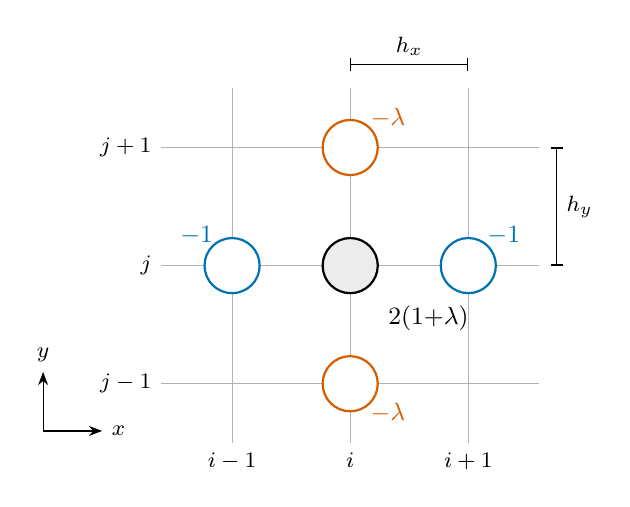
\begin{tikzpicture}[scale=1.5,
      nd/.style={circle, draw, thick, minimum size=7mm, inner sep=0pt, fill=white},
      wt/.style={font=\small}]
    \draw[gray!60] (-1.6,0) -- (1.6,0);
    \draw[gray!60] (-1.6,1) -- (1.6,1);
    \draw[gray!60] (-1.6,-1) -- (1.6,-1);
    \draw[gray!60] (-1,-1.5) -- (-1,1.5);
    \draw[gray!60] (0,-1.5) -- (0,1.5);
    \draw[gray!60] (1,-1.5) -- (1,1.5);
    \node[nd, draw=cdiag, fill=gray!15] at (0,0) {};
    \node[nd, draw=cx] at (-1,0) {};
    \node[nd, draw=cx] at (1,0) {};
    \node[nd, draw=cy] at (0,1) {};
    \node[nd, draw=cy] at (0,-1) {};
    \node[wt, cdiag, anchor=north west] at (0.24,-0.26) {$2(1{+}\lambda)$};
    \node[wt, cx] at (-1.3,0.25) {$-1$};
    \node[wt, cx] at (1.3,0.25) {$-1$};
    \node[wt, cy] at (0.32,1.25) {$-\lambda$};
    \node[wt, cy] at (0.32,-1.25) {$-\lambda$};
    \node[font=\footnotesize, below] at (-1,-1.5) {$i-1$};
    \node[font=\footnotesize, below] at (0,-1.5) {$i$};
    \node[font=\footnotesize, below] at (1,-1.5) {$i+1$};
    \node[font=\footnotesize, left] at (-1.6,1) {$j+1$};
    \node[font=\footnotesize, left] at (-1.6,0) {$j$};
    \node[font=\footnotesize, left] at (-1.6,-1) {$j-1$};
    \draw[|-|] (0,1.7) -- node[above, font=\footnotesize] {$h_x$} (1,1.7);
    \draw[|-|] (1.75,0) -- node[right, font=\footnotesize] {$h_y$} (1.75,1);
    \draw[-{Stealth}] (-2.6,-1.4) -- (-2.1,-1.4) node[right, font=\footnotesize] {$x$};
    \draw[-{Stealth}] (-2.6,-1.4) -- (-2.6,-0.9) node[above, font=\footnotesize] {$y$};
  \end{tikzpicture}
  \caption{Five-point stencil of the central-difference scheme~\eqref{eq:stencil} at node
    $(i,j)$ with the weights of the neighbouring nodes. For an isotropic medium on a
    square mesh, $\lambda = 1$.}
  \label{fig:stencil}
\end{figure}

\begin{remark}\label{rem:meanvalue}
  For an isotropic medium on a square mesh ($P = 1$, $h_x = h_y$), we have $\lambda = 1$,
  and~\eqref{eq:stencil} states that $\rho_{i,j}$ equals the arithmetic mean of its four
  neighbours. This discrete mean-value property implies a discrete maximum principle: no
  interior node can exceed all of its neighbours, so extrema of the discrete solution lie
  on the boundary, exactly as for harmonic functions. Moreover, the truncation
  error~\eqref{eq:truncation} vanishes for polynomials of degree at most three in each
  variable, so that linear concentration profiles, as expected in the test problems of
  Part~II, are reproduced exactly up to round-off.
\end{remark}

\subsection{Node numbering (Task 2.2a)}\label{sec:numbering}

\begin{task}{2.2}
  A rectangular domain whose edges are aligned with the principal axes of the diffusion
  tensor is discretized by $5\times5$ nodes. Write the scheme of Task~2.1 as a linear
  system of equations.
  \begin{enumerate}
    \item[(a)] Number the nodes row-wise from the top left (node~1) to the bottom right
      (node~25), and sketch the mapping between the indices $(i,j)$ and the node number
      for a general mesh of $N \times M$ nodes.
    \item[(b)] Sketch the interior part of the coefficient matrix, whose entries follow from
      the factors of the nodal values in the scheme, and explain the difficulties that
      arise at the boundaries.
  \end{enumerate}
\end{task}

To write the discrete equations as a linear system, the two-dimensional node indices
$(i,j)$ must be mapped onto a single index $k$ of a solution vector. Following the
script, we number the nodes row-wise, starting at the top left node and ending at the
bottom right node (\cref{fig:numbering}). For a mesh of $N \times M$ nodes, that is
$N_x = N$ nodes per row and $N_y = M$ rows, the top row ($j = M$) receives the numbers
$1$ to $N$, the next row the numbers $N + 1$ to $2N$, and so forth. The mapping and its
inverse are
\begin{equation}\label{eq:mapping}
  k(i,j) = (M - j)\,N + i,
  \qquad
  i = 1 + \bigl((k - 1) \bmod N\bigr),
  \qquad
  j = M - \left\lfloor \frac{k - 1}{N} \right\rfloor,
\end{equation}
with $k = 1, \dots, NM$. The four neighbours of node $k$ follow directly from
\eqref{eq:mapping}:
\begin{equation}\label{eq:neighbours}
  (i \pm 1, j) \;\mapsto\; k \pm 1,
  \qquad
  (i, j \pm 1) \;\mapsto\; k \mp N.
\end{equation}
Horizontal neighbours are adjacent in the vector, and vertical neighbours are $N$
positions apart. In a zero-based implementation with the row index $r = M - j$ counted
from the top and $i' = i - 1$, the mapping reads $k' = rN + i'$. This is the row-major
(C) ordering of NumPy, so that the solution vector can be reshaped directly into an
$M \times N$ array whose first row is the top of the domain.

\begin{figure}[ht]
  \centering
  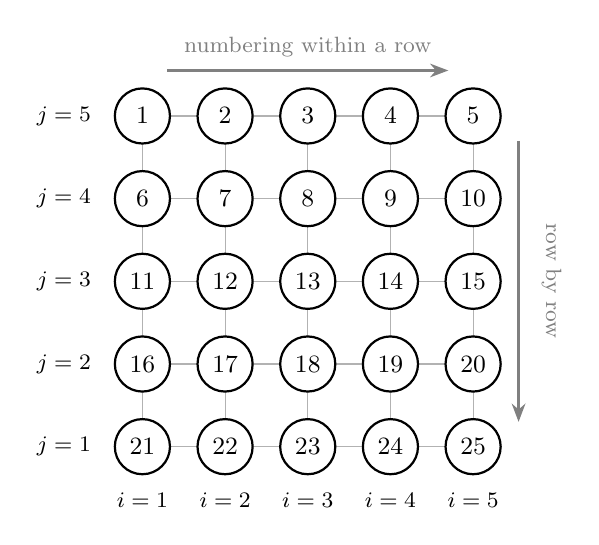
\begin{tikzpicture}[scale=1.05,
      nd/.style={circle, draw, thick, minimum size=7mm, inner sep=0pt, font=\small}]
    \foreach \r in {0,...,4} {
      \draw[gray!60] (0,-\r) -- (4,-\r);
      \draw[gray!60] (\r,0) -- (\r,-4);
    }
    \foreach \r in {0,...,4} {
      \foreach \i in {0,...,4} {
        \pgfmathtruncatemacro{\k}{5*\r + \i + 1}
        \node[nd, fill=white] at (\i,-\r) {\k};
      }
    }
    \foreach \i in {1,...,5} {
      \node[font=\footnotesize] at (\i-1,-4.65) {$i=\i$};
    }
    \foreach \r in {0,...,4} {
      \pgfmathtruncatemacro{\j}{5 - \r}
      \node[font=\footnotesize] at (-0.95,-\r) {$j=\j$};
    }
    \draw[-{Stealth}, thick, gray] (0.3,0.55) -- (3.7,0.55);
    \draw[-{Stealth}, thick, gray] (4.55,-0.3) -- (4.55,-3.7);
    \node[font=\footnotesize, gray, above] at (2,0.6) {numbering within a row};
    \node[font=\footnotesize, gray, rotate=-90] at (4.95,-2) {row by row};
  \end{tikzpicture}
  \caption{Row-wise numbering of a $5 \times 5$ mesh ($N = M = 5$) from the top left node
    ($k = 1$) to the bottom right node ($k = 25$). Node $(i,j)$ receives the number
    $k = (M - j)N + i$; for example, the centre node $(3,3)$ is node $13$.}
  \label{fig:numbering}
\end{figure}

\subsection{Coefficient matrix without boundary conditions (Task 2.2b)}\label{sec:inner}

Applying the stencil~\eqref{eq:stencil} to node $k$ and using~\eqref{eq:neighbours}
gives the $k$-th row of the linear system,
\begin{equation}\label{eq:row}
  -\lambda\,\rho_{k-N} - \rho_{k-1} + 2(1 + \lambda)\,\rho_k - \rho_{k+1}
  - \lambda\,\rho_{k+N} = 0.
\end{equation}
Each row therefore contains at most five non-zero coefficients,
\begin{equation}\label{eq:coefficients}
  c_{k,k} = 2(1 + \lambda),
  \qquad
  c_{k,k\pm1} = -1,
  \qquad
  c_{k,k\pm N} = -\lambda,
\end{equation}
located on the main diagonal, on the first sub- and superdiagonals and on the two
diagonals at distance $N$. For the $5\times5$ mesh, the inner part of the matrix consists of
the rows of the nine interior nodes $k \in \{7, 8, 9, 12, 13, 14, 17, 18, 19\}$; for
instance, the row of the centre node reads
\begin{equation}\label{eq:row13}
  -\lambda\,\rho_{8} - \rho_{12} + 2(1 + \lambda)\,\rho_{13} - \rho_{14}
  - \lambda\,\rho_{18} = 0.
\end{equation}
\Cref{fig:sparsity} shows the resulting sparsity pattern of the $25 \times 25$
coefficient matrix. The interior rows are complete, while the rows of the 16 boundary
nodes cannot be formed from the stencil alone. Three difficulties arise in these rows.
\begin{enumerate}
  \item \emph{Missing neighbours.} At boundary nodes the stencil reaches nodes outside the
    mesh, with $i = 0$, $i = N + 1$, $j = 0$ or $j = M + 1$, which have no index. For the
    top and bottom rows the indices $k \mp N$ fall outside $\{1, \dots, NM\}$.
  \item \emph{Wrap-around of the numbering.} For a node on the right edge, $k + 1$ is the
    first node of the next row on the left edge (for example $5 \to 6$), and for a node
    on the left edge, $k - 1$ is the last node of the previous row. A naive assembly
    along continuous diagonals therefore couples opposite edges of the domain, which is
    unphysical; the corresponding entries of the first sub- and superdiagonals must be
    zero.
  \item \emph{Missing information.} The $(N - 2)(M - 2)$ interior equations cannot
    determine $NM$ unknowns. Without boundary conditions, the homogeneous system admits
    every discrete harmonic function, including all constants and linear functions, as a
    solution. This reflects the elliptic character of the problem
    (\cref{sec:classification}): the solution is determined by data on the whole
    boundary, which the boundary conditions of \cref{sec:bc} supply.
\end{enumerate}

\begin{figure}[ht]
  \centering
  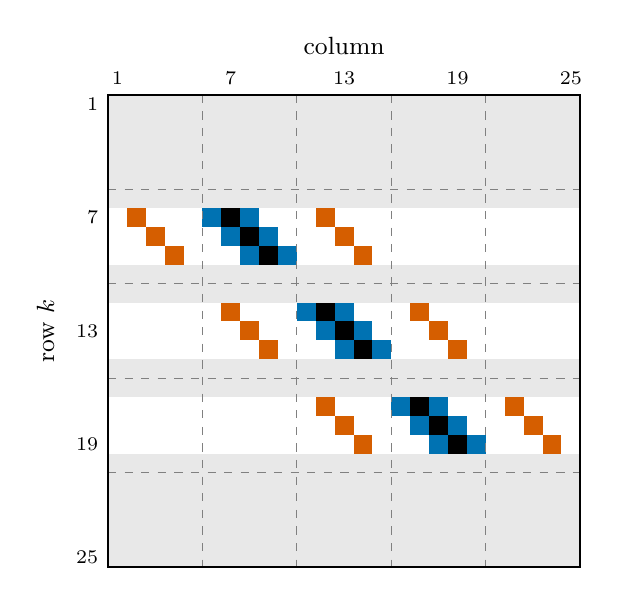
\begin{tikzpicture}[x=0.24cm, y=0.24cm]
    \foreach \k in {1,2,3,4,5,6,10,11,15,16,20,21,22,23,24,25} {
      \fill[gray!18] (0,-\k) rectangle (25,-\k+1);
    }
    \foreach \k in {7,8,9,12,13,14,17,18,19} {
      \fill[cdiag] (\k-1,-\k) rectangle (\k,-\k+1);
      \fill[cx] (\k-2,-\k) rectangle (\k-1,-\k+1);
      \fill[cx] (\k,-\k) rectangle (\k+1,-\k+1);
      \fill[cy] (\k-6,-\k) rectangle (\k-5,-\k+1);
      \fill[cy] (\k+4,-\k) rectangle (\k+5,-\k+1);
    }
    \foreach \b in {5,10,15,20} {
      \draw[gray, dashed] (\b,0) -- (\b,-25);
      \draw[gray, dashed] (0,-\b) -- (25,-\b);
    }
    \draw[thick] (0,0) rectangle (25,-25);
    \foreach \k in {1,7,13,19,25} {
      \node[font=\scriptsize, left] at (0,-\k+0.5) {\k};
      \node[font=\scriptsize, above] at (\k-0.5,0) {\k};
    }
    \node[font=\small, rotate=90] at (-3.3,-12.5) {row $k$};
    \node[font=\small] at (12.5,2.6) {column};
  \end{tikzpicture}
  \caption{Sparsity pattern of the $25 \times 25$ coefficient matrix of the $5 \times 5$
    mesh before boundary conditions are applied. Black: diagonal $2(1 + \lambda)$; blue:
    horizontal neighbours $-1$ at distance $1$; orange: vertical neighbours $-\lambda$ at
    distance $N = 5$. Grey rows belong to boundary nodes, for which the stencil is
    incomplete. Dashed lines delimit the $5\times5$ blocks that correspond to mesh rows.}
  \label{fig:sparsity}
\end{figure}

% ===============================================================
\section{Boundary conditions}\label{sec:bc}
% ===============================================================

Following the script, we prescribe the concentration on the upper and lower boundaries
(Dirichlet conditions $\rhoUpper$ and $\rhoLower$) and the diffusion flux on the left and right
boundaries (Neumann conditions $\jleft$ and $\jright$). \Cref{fig:bc} shows the
configuration for the $5 \times 5$ mesh. The nodes on the upper and lower boundaries,
labelled A to E and F to J, carry known values and are no longer unknowns. The remaining
$N(M - 2) = 15$ nodes are renumbered row-wise from 1 to 15, so that node $(i,j)$ with
$2 \le j \le M - 1$ receives the number $k = (M - 1 - j)N + i$.

\begin{figure}[ht]
  \centering
  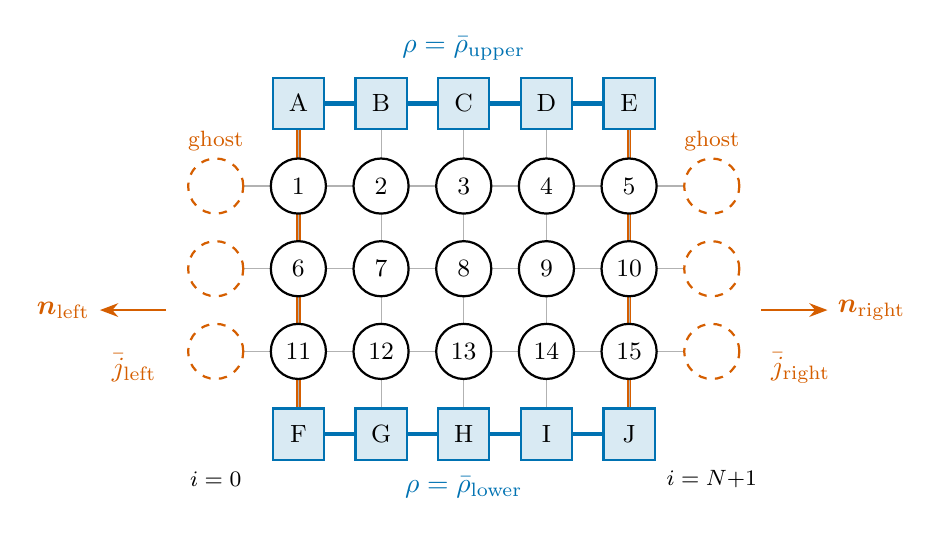
\begin{tikzpicture}[scale=1.05,
      nd/.style={circle, draw, thick, minimum size=7mm, inner sep=0pt, font=\small, fill=white},
      dn/.style={rectangle, draw=cdir, fill=cdir!15, thick, minimum size=6.5mm, inner sep=0pt, font=\small},
      gn/.style={circle, draw=cneu, dashed, thick, minimum size=7mm, inner sep=0pt, fill=white}]
    % domain
    \draw[line width=1.6pt, cdir] (0,1) -- (4,1);
    \draw[line width=1.6pt, cdir] (0,-3) -- (4,-3);
    \draw[line width=1.6pt, cneu] (0,1) -- (0,-3);
    \draw[line width=1.6pt, cneu] (4,1) -- (4,-3);
    % mesh lines
    \foreach \r in {0,1,2} {
      \draw[gray!60] (-1,-\r) -- (5,-\r);
    }
    \foreach \i in {0,...,4} {
      \draw[gray!60] (\i,1) -- (\i,-3);
    }
    % Dirichlet nodes
    \foreach \i/\l in {0/A,1/B,2/C,3/D,4/E} {
      \node[dn] at (\i,1) {\l};
    }
    \foreach \i/\l in {0/F,1/G,2/H,3/I,4/J} {
      \node[dn] at (\i,-3) {\l};
    }
    % ghost nodes
    \foreach \r in {0,1,2} {
      \node[gn] at (-1,-\r) {};
      \node[gn] at (5,-\r) {};
    }
    % unknowns
    \foreach \r in {0,1,2} {
      \foreach \i in {0,...,4} {
        \pgfmathtruncatemacro{\k}{5*\r + \i + 1}
        \node[nd] at (\i,-\r) {\k};
      }
    }
    % labels
    \node[cdir, above] at (2,1.4) {$\rho = \rhoUpper$};
    \node[cdir, below] at (2,-3.4) {$\rho = \rhoLower$};
    \draw[-{Stealth}, thick, cneu] (-1.6,-1.5) -- (-2.4,-1.5)
      node[left] {$\bn_{\mathrm{left}}$};
    \draw[-{Stealth}, thick, cneu] (5.6,-1.5) -- (6.4,-1.5)
      node[right] {$\bn_{\mathrm{right}}$};
    \node[cneu, left] at (-1.6,-2.2) {$\jleft$};
    \node[cneu, right] at (5.6,-2.2) {$\jright$};
    \node[font=\footnotesize, cneu] at (-1,0.55) {ghost};
    \node[font=\footnotesize, cneu] at (5,0.55) {ghost};
    \node[font=\footnotesize] at (-1,-3.55) {$i=0$};
    \node[font=\footnotesize] at (5,-3.55) {$i=N{+}1$};
  \end{tikzpicture}
  \caption{Boundary conditions and discretization of the $5 \times 5$ mesh. Squares
    (blue): Dirichlet nodes A to E ($\rhoUpper$) and F to J ($\rhoLower$), whose values are
    known. Circles: the 15 unknown nodes, numbered row-wise. Dashed circles (orange):
    ghost nodes outside the domain, used to impose the prescribed fluxes $\jleft$ and
    $\jright$ on the left and right boundaries with outward normals $\bn_{\mathrm{left}}$
    and $\bn_{\mathrm{right}}$.}
  \label{fig:bc}
\end{figure}

\subsection{Dirichlet boundary conditions (Task 3.1)}\label{sec:dirichlet}

\begin{task}{3.1}
  The concentrations $\rhoUpper$ and $\rhoLower$ are prescribed on the upper and lower
  boundaries, so the nodes there are no longer unknowns (\cref{fig:bc}). State which nodes
  enter the scheme at node~3, derive the corresponding linear equation using that
  $\rho_C$ is known, and collect all known quantities on the right-hand side.
\end{task}

Node~3 is the mesh node $(i,j) = (3,4)$ in the top row of unknowns. The stencil at this
node involves its left and right neighbours 2 and 4, its lower neighbour 8 and its upper
neighbour C, which is the Dirichlet node $(3,5)$ with the known value
$\rho_C = \rhoUpper$. Equation~\eqref{eq:stencil} at node~3 reads
\begin{equation}\label{eq:node3-raw}
  2(1 + \lambda)\,\rho_3 - \rho_2 - \rho_4 - \lambda\,\rho_8 - \lambda\,\rho_C = 0.
\end{equation}
Moving the known value to the right-hand side gives
\begin{equation}\label{eq:node3}
  \boxed{\;
    -\rho_2 + 2(1 + \lambda)\,\rho_3 - \rho_4 - \lambda\,\rho_8 = \lambda\,\rhoUpper.
  \;}
\end{equation}
The Dirichlet node thus disappears from the unknowns and contributes $\lambda\,\rhoUpper$
to the right-hand side; its coefficient is removed from the row. The same holds for
nodes 1 to 5 with the upper boundary and for nodes 11 to 15 with the lower boundary,
where $\lambda\,\rhoLower$ enters. Eliminating the Dirichlet nodes, rather than keeping them
as unknowns with trivial equations $\rho_C = \rhoUpper$, reduces the size of the system and
preserves the structure of the matrix discussed in \cref{sec:properties}.

\subsection{Neumann boundary conditions (Task 3.2)}\label{sec:neumann}

\begin{task}{3.2}
  The diffusion fluxes $\jleft$ and $\jright$ are prescribed on the left and right
  boundaries, measured along the outward normal, so that a negative value denotes flux
  into the domain. Discretize Fick's first law by finite differences and use it to express
  the ghost nodes outside the domain through known quantities, taking the direction of the
  flux into account. Derive the equation for node~10 with all known quantities on the
  right-hand side.
\end{task}

\paragraph{Prescribed flux.} On the left and right boundaries the normal component of the
flux, $\bar{j} = \bj\cdot\bn$, is prescribed, where $\bn$ is the outward unit normal
($\bn_{\mathrm{left}} = -\be_x$, $\bn_{\mathrm{right}} = +\be_x$). By this convention,
$\bar{j} < 0$ if the flux is directed into the domain and $\bar{j} > 0$ if it leaves the
domain. With Fick's first law for an isotropic medium, $\bj\cdot\bn =
-D\,\partial\rho/\partial n$, so that
\begin{equation}\label{eq:neumann}
  \frac{\partial\rho}{\partial n} = -\frac{\bar{j}}{D}
  \quad\Longrightarrow\quad
  \partial_x\rho\big|_{\mathrm{right}} = -\frac{\jright}{D},
  \qquad
  \partial_x\rho\big|_{\mathrm{left}} = +\frac{\jleft}{D}.
\end{equation}
The sign difference between the two boundaries reflects the opposite orientation of the
outward normals: an outward flux at the right boundary requires a concentration that
decreases towards the boundary, whereas at the left boundary it requires a
concentration that increases away from it.

\paragraph{Ghost nodes.} The boundary nodes on the left and right edges are unknowns, but
their stencil reaches the nodes $(0, j)$ and $(N + 1, j)$ outside the domain. We introduce
these \emph{ghost nodes} as auxiliary values and eliminate them by discretizing
\eqref{eq:neumann} with a central difference centred on the boundary node,
\begin{align}
  \frac{\rho_{N+1,j} - \rho_{N-1,j}}{2h_x} &= -\frac{\jright}{D}
  &&\Longrightarrow&
  \rho_{N+1,j} &= \rho_{N-1,j} - \frac{2h_x}{D}\,\jright,
  \label{eq:ghost-right}\\
  \frac{\rho_{2,j} - \rho_{0,j}}{2h_x} &= +\frac{\jleft}{D}
  &&\Longrightarrow&
  \rho_{0,j} &= \rho_{2,j} - \frac{2h_x}{D}\,\jleft.
  \label{eq:ghost-left}
\end{align}
Both boundaries thus obey the same rule: the ghost value equals the value at the mirror
node inside the domain, shifted by $-2h_x\bar{j}/D$. A central difference is accurate to
$\bigO{h_x^2}$, consistent with the interior scheme~\eqref{eq:truncation}. A one-sided
difference such as $(\rho_{N,j} - \rho_{N-1,j})/h_x$ would introduce an $\bigO{h_x}$
error at the boundary and degrade the accuracy of the solution.

\paragraph{Equation for node 10.} Node~10 is the mesh node $(5,3)$ on the right boundary.
Its neighbours are node~9 to the left, node~5 above, node~15 below and the ghost node
$(6,3)$ to the right. The stencil~\eqref{eq:stencil} gives
\begin{equation}\label{eq:node10-raw}
  2(1 + \lambda)\,\rho_{10} - \rho_9 - \rho_{6,3} - \lambda\,\rho_5 - \lambda\,\rho_{15} = 0.
\end{equation}
Substituting the ghost value $\rho_{6,3} = \rho_9 - 2h_x\jright/D$
from~\eqref{eq:ghost-right} and moving the known flux to the right-hand side yields
\begin{equation}\label{eq:node10}
  \boxed{\;
    -\lambda\,\rho_5 - 2\rho_9 + 2(1 + \lambda)\,\rho_{10} - \lambda\,\rho_{15}
    = -\frac{2h_x}{D}\,\jright.
  \;}
\end{equation}
The coupling to the interior neighbour doubles because the ghost node is a reflected copy
of node~9. The sign of the right-hand side is physically consistent: an outward flux
($\jright > 0$) lowers the concentration at the boundary. The nodes 1, 5, 11 and 15 at the
corners of the unknown region combine both types of boundary condition. For node~1, for
example,
\begin{equation}\label{eq:node1}
  2(1 + \lambda)\,\rho_1 - 2\rho_2 - \lambda\,\rho_6
  = \lambda\,\rhoUpper - \frac{2h_x}{D}\,\jleft.
\end{equation}

\begin{remark}\label{rem:pureneumann}
  The Dirichlet conditions are essential for uniqueness. If fluxes were prescribed on the
  entire boundary, any constant could be added to a solution, the matrix would be
  singular, and a solution would exist only if the prescribed fluxes satisfied the
  compatibility condition $\oint_{\partial\Omega}\bar{j}\,\mathrm{d}s = 0$, which states
  that the net flux out of the domain vanishes in the stationary state.
\end{remark}

% ===============================================================
\section{Linear system}\label{sec:system}
% ===============================================================

\subsection{Assembly (Task 4.1)}\label{sec:assembly}

\begin{task}{4.1}
  Assemble the complete linear system $\bA\brho = \bb_\rho - \bb_j$, in which the two
  right-hand-side vectors carry the prescribed concentrations and fluxes. Identify which
  entries belong to the upper, lower, left and right boundaries and which to interior
  nodes.
\end{task}

Collecting the equations of all 15 unknown nodes, with interior rows of the
form~\eqref{eq:row}, Dirichlet contributions as in~\eqref{eq:node3} and Neumann
contributions as in~\eqref{eq:node10}, yields the linear system
\begin{equation}\label{eq:system}
  \bA\,\brho = \bb_\rho - \bb_j,
\end{equation}
where $\brho = (\rho_1, \dots, \rho_{15})^{\mathsf{T}}$ is the vector of unknowns,
$\bb_\rho$ contains the Dirichlet data and $\bb_j$ the Neumann data. For an isotropic
medium on a square mesh ($\lambda = 1$, $h_x = h_y = h$), the system reads
\begingroup
\setlength{\arraycolsep}{2.4pt}
\footnotesize
\begin{equation}\label{eq:system-explicit}
  \underbrace{\begin{bmatrix}
     4 & -2 & \cdot & \cdot & \cdot & -1 & \cdot & \cdot & \cdot & \cdot & \cdot & \cdot & \cdot & \cdot & \cdot \\
    -1 &  4 & -1 & \cdot & \cdot & \cdot & -1 & \cdot & \cdot & \cdot & \cdot & \cdot & \cdot & \cdot & \cdot \\
    \cdot & -1 &  4 & -1 & \cdot & \cdot & \cdot & -1 & \cdot & \cdot & \cdot & \cdot & \cdot & \cdot & \cdot \\
    \cdot & \cdot & -1 &  4 & -1 & \cdot & \cdot & \cdot & -1 & \cdot & \cdot & \cdot & \cdot & \cdot & \cdot \\
    \cdot & \cdot & \cdot & -2 &  4 & \cdot & \cdot & \cdot & \cdot & -1 & \cdot & \cdot & \cdot & \cdot & \cdot \\
    -1 & \cdot & \cdot & \cdot & \cdot &  4 & -2 & \cdot & \cdot & \cdot & -1 & \cdot & \cdot & \cdot & \cdot \\
    \cdot & -1 & \cdot & \cdot & \cdot & -1 &  4 & -1 & \cdot & \cdot & \cdot & -1 & \cdot & \cdot & \cdot \\
    \cdot & \cdot & -1 & \cdot & \cdot & \cdot & -1 &  4 & -1 & \cdot & \cdot & \cdot & -1 & \cdot & \cdot \\
    \cdot & \cdot & \cdot & -1 & \cdot & \cdot & \cdot & -1 &  4 & -1 & \cdot & \cdot & \cdot & -1 & \cdot \\
    \cdot & \cdot & \cdot & \cdot & -1 & \cdot & \cdot & \cdot & -2 &  4 & \cdot & \cdot & \cdot & \cdot & -1 \\
    \cdot & \cdot & \cdot & \cdot & \cdot & -1 & \cdot & \cdot & \cdot & \cdot &  4 & -2 & \cdot & \cdot & \cdot \\
    \cdot & \cdot & \cdot & \cdot & \cdot & \cdot & -1 & \cdot & \cdot & \cdot & -1 &  4 & -1 & \cdot & \cdot \\
    \cdot & \cdot & \cdot & \cdot & \cdot & \cdot & \cdot & -1 & \cdot & \cdot & \cdot & -1 &  4 & -1 & \cdot \\
    \cdot & \cdot & \cdot & \cdot & \cdot & \cdot & \cdot & \cdot & -1 & \cdot & \cdot & \cdot & -1 &  4 & -1 \\
    \cdot & \cdot & \cdot & \cdot & \cdot & \cdot & \cdot & \cdot & \cdot & -1 & \cdot & \cdot & \cdot & -2 &  4
  \end{bmatrix}}_{\bA}
  \begin{bmatrix}
    \rho_1 \\ \rho_2 \\ \rho_3 \\ \rho_4 \\ \rho_5 \\ \rho_6 \\ \rho_7 \\ \rho_8 \\
    \rho_9 \\ \rho_{10} \\ \rho_{11} \\ \rho_{12} \\ \rho_{13} \\ \rho_{14} \\ \rho_{15}
  \end{bmatrix}
  =
  \underbrace{\begin{bmatrix}
    \rhoUpper \\ \rhoUpper \\ \rhoUpper \\ \rhoUpper \\ \rhoUpper \\
    0 \\ 0 \\ 0 \\ 0 \\ 0 \\
    \rhoLower \\ \rhoLower \\ \rhoLower \\ \rhoLower \\ \rhoLower
  \end{bmatrix}}_{\bb_\rho}
  -
  \underbrace{\frac{2h}{D}
  \begin{bmatrix}
    \jleft \\ 0 \\ 0 \\ 0 \\ \jright \\
    \jleft \\ 0 \\ 0 \\ 0 \\ \jright \\
    \jleft \\ 0 \\ 0 \\ 0 \\ \jright
  \end{bmatrix}}_{\bb_j},
\end{equation}
\endgroup
where dots denote zeros. For general $\lambda$ and mesh spacing, the matrix has the block
structure
\begin{equation}\label{eq:block}
  \bA =
  \begin{bmatrix}
    \bT & -\lambda\bI & \mathbf{0} \\
    -\lambda\bI & \bT & -\lambda\bI \\
    \mathbf{0} & -\lambda\bI & \bT
  \end{bmatrix},
  \qquad
  \bT =
  \begin{bmatrix}
    d & -2 & & & \\
    -1 & d & -1 & & \\
    & -1 & d & -1 & \\
    & & -1 & d & -1 \\
    & & & -2 & d
  \end{bmatrix},
  \qquad
  d \coloneqq 2(1 + \lambda),
\end{equation}
where $\bI$ is the $5 \times 5$ identity, and the right-hand side generalizes to
$\bb_\rho = \lambda\,(\rhoUpper\bm{1}_5,\, \bm{0}_5,\, \rhoLower\bm{1}_5)^{\mathsf{T}}$ and
$\bb_j = (2h_x/D)\,(\jleft, 0, 0, 0, \jright, \dots)^{\mathsf{T}}$, with $\bm{1}_5$ and
$\bm{0}_5$ the vectors of five ones and five zeros. Each block row of $\bA$ corresponds to
one row of unknown nodes, and each block $\bT$ couples the nodes within that row.
\Cref{tab:rows} summarizes how the boundaries enter the system. The first column on the
right-hand side, $\bb_\rho$, carries the Dirichlet data of the upper and lower boundaries;
the second, $\bb_j$, carries the Neumann data of the left and right boundaries.

\begin{table}[ht]
  \centering
  \caption{Contribution of each boundary to the rows of the linear
    system~\eqref{eq:system-explicit}.}
  \label{tab:rows}
  \begin{tabularx}{\linewidth}{llX}
    \toprule
    Boundary & Rows $k$ & Effect on the system \\
    \midrule
    Upper (Dirichlet) & 1 to 5 & No coupling to a block above; entry $\lambda\rhoUpper$ in $\bb_\rho$ \\
    Lower (Dirichlet) & 11 to 15 & No coupling to a block below; entry $\lambda\rhoLower$ in $\bb_\rho$ \\
    Left (Neumann) & 1, 6, 11 & Coefficient $-2$ at column $k + 1$; entry $2h_x\jleft/D$ in $\bb_j$ \\
    Right (Neumann) & 5, 10, 15 & Coefficient $-2$ at column $k - 1$; entry $2h_x\jright/D$ in $\bb_j$ \\
    Interior & 7, 8, 9 & Full stencil~\eqref{eq:row}; zero right-hand side \\
    \bottomrule
  \end{tabularx}
\end{table}

\subsection{Properties of the coefficient matrix (Task 4.2)}\label{sec:properties}

\begin{task}{4.2}
  Discuss the numerical properties of the coefficient matrix, such as its structure, and
  the parameters that determine its shape.
\end{task}

For a mesh of $N_x \times N_y$ nodes, $\bA$ is a square matrix of dimension
$n = N_x(N_y - 2)$ with the following properties.

\paragraph{Sparsity and band structure.} Each row contains at most five non-zero entries,
so $\bA$ has at most $5n$ non-zeros out of $n^2$ entries. The matrix is pentadiagonal with
outer diagonals at distance $N_x$, so its half-bandwidth equals $N_x$. Equivalently, it is
block tridiagonal with $N_y - 2$ tridiagonal diagonal blocks $\bT$ of size $N_x$ and
off-diagonal blocks $-\lambda\bI$. Storage in a sparse format therefore requires
$\bigO{n}$ memory, and a banded direct solver requires $\bigO{nN_x^2}$ operations, since
fill-in during the factorization is confined to the band~\citep{golub2013}.

\paragraph{Diagonal dominance and regularity.} In every row the diagonal entry equals the
sum of the magnitudes of the off-diagonal entries: $2(1 + \lambda) = 1 + 1 + \lambda +
\lambda$ for interior rows and $2(1 + \lambda) = 2 + \lambda + \lambda$ for Neumann rows.
In the $2N_x$ rows adjacent to a Dirichlet boundary one off-diagonal entry has been
removed, and the inequality is strict. Since the mesh is connected, $\bA$ is irreducible.
An irreducible matrix that is weakly diagonally dominant in all rows and strictly
diagonally dominant in at least one row is nonsingular~\citep{varga2000}. The discrete
problem therefore has a unique solution for all boundary data.

\paragraph{M-matrix and monotonicity.} The diagonal entries of $\bA$ are positive and the
off-diagonal entries are non-positive. Together with the irreducible diagonal dominance,
this makes $\bA$ a nonsingular M-matrix, whose inverse is entrywise
non-negative~\citep{varga2000}. Two physically meaningful consequences follow. First,
non-negative boundary concentrations combined with non-positive (inward) fluxes give
$\bb_\rho - \bb_j \ge 0$ and hence a non-negative concentration everywhere. Second, the
solution depends monotonically on the data: raising a boundary concentration never lowers
the concentration at any node. This is the discrete counterpart of the maximum
principle.

\paragraph{Symmetry and spectrum.} The matrix is not symmetric, because each Neumann row
couples to its interior neighbour with the coefficient $-2$, while the interior neighbour
couples back with $-1$ (for example $a_{1,2} = -2$ but $a_{2,1} = -1$). The asymmetry is
removed by halving the Neumann rows: with $\bW = \operatorname{diag}(w_k)$, where $w_k =
1/2$ for $k$ on the left or right boundary and $w_k = 1$ otherwise, the matrix $\bS =
\bW\bA$ is symmetric. As a symmetric, diagonally dominant matrix with positive diagonal,
$\bS$ is positive semidefinite by Gershgorin's theorem, and since it is nonsingular, it is
positive definite. Because $\bA = \bW^{-1}\bS$ is similar to the symmetric positive
definite matrix $\bW^{-1/2}\bS\,\bW^{-1/2}$, all eigenvalues of $\bA$ are real and
positive. The symmetrized system $\bS\brho = \bW(\bb_\rho - \bb_j)$ can therefore be
solved with the Cholesky factorization or the conjugate gradient method.

\paragraph{Conditioning.} The smallest eigenvalue of $\bA$ scales as $\bigO{h^2}$ and the
largest remains bounded, so that the spectral condition number grows as $\bigO{h^{-2}}$
under mesh refinement~\citep{leveque2007}. Fine meshes thus require more iterations of
iterative solvers, and round-off errors are amplified more strongly.

\paragraph{Parameters that influence the shape of the matrix.}
\begin{itemize}
  \item The number of nodes per row, $N_x$, sets the size of the blocks and the distance
    of the outer diagonals from the main diagonal, that is, the bandwidth.
  \item The number of rows, $N_y$, sets the number of block rows, which is $N_y - 2$ after
    elimination of the Dirichlet nodes.
  \item The numbering scheme determines which dimension sets the bandwidth. Column-wise
    numbering would yield the half-bandwidth $N_y - 2$ instead of $N_x$, so the cost of a
    banded solver is minimized by numbering along the shorter side of the mesh.
  \item The type of boundary condition modifies the boundary rows: Dirichlet conditions
    remove rows and columns and make the adjacent rows strictly diagonally dominant;
    Neumann conditions double the coupling to the interior neighbour and break the
    symmetry.
  \item The weight $\lambda = P h_x^2/h_y^2$, which depends on the anisotropy and on the
    domain size and node numbers through $h_x$ and $h_y$, changes the values of the
    entries but not the sparsity pattern.
  \item If the principal axes of $\bD$ were not aligned with the mesh, the mixed
    derivative in~\eqref{eq:fick2-expanded} would require the diagonal neighbours
    $(i \pm 1, j \pm 1)$, giving a nine-point stencil with four additional diagonals at
    distances $N_x \pm 1$.
\end{itemize}

% ===============================================================
\section{Summary}\label{sec:summary}
% ===============================================================

We have derived Fick's second law for an anisotropic two-dimensional medium from the
continuity equation and Fick's first law, and shown that it is parabolic, while its
stationary limit is elliptic. In the principal axes of the diffusion tensor, stationary
diffusion obeys $\partial^2_{xx}\rho + P\,\partial^2_{yy}\rho = 0$, where $P$ is the ratio
of the principal diffusivities, and a rescaling of one coordinate maps this equation onto
the Laplace equation. A second-order central-difference scheme on an equidistant mesh,
combined with row-wise numbering, elimination of Dirichlet nodes and ghost nodes for the
Neumann conditions, leads to the linear system~\eqref{eq:system}. Its coefficient matrix
is sparse, pentadiagonal and block tridiagonal, irreducibly diagonally dominant and a
nonsingular M-matrix with real positive eigenvalues; the asymmetry caused by the Neumann
rows is removed by a diagonal scaling. These properties guarantee a unique discrete
solution that is non-negative for physically admissible data and depends monotonically on
them, and they permit efficient sparse direct or iterative solvers. Part~II implements this system for arbitrary domain sizes, node
numbers and boundary values, and verifies it against the test problems of Task~5.

% ===============================================================
\begin{thebibliography}{99}
% ===============================================================

\bibitem{script}
Institute of Materials Simulation (WW8),
``Theoretical foundations and simulation of diffusion processes by use of finite
differences,''
Materials Simulation Practical No.~1, tutorial script,
Friedrich-Alexander-Universit\"at Erlangen-N\"urnberg.

\bibitem{fick1855}
A.~Fick,
``Ueber Diffusion,''
\textit{Annalen der Physik},
vol.~170, no.~1, pp.~59--86, 1855.

\bibitem{crank1975}
J.~Crank,
\textit{The Mathematics of Diffusion},
2nd~ed.,
Clarendon Press, Oxford, 1975.

\bibitem{onsager1931}
L.~Onsager,
``Reciprocal relations in irreversible processes.~I,''
\textit{Physical Review},
vol.~37, no.~4, pp.~405--426, 1931.

\bibitem{nye1985}
J.~F.~Nye,
\textit{Physical Properties of Crystals: Their Representation by Tensors and Matrices},
Oxford University Press, Oxford, 1985.

\bibitem{evans2010}
L.~C.~Evans,
\textit{Partial Differential Equations},
2nd~ed.,
American Mathematical Society, Providence, RI, 2010.

\bibitem{leveque2007}
R.~J.~LeVeque,
\textit{Finite Difference Methods for Ordinary and Partial Differential Equations:
Steady-State and Time-Dependent Problems},
SIAM, Philadelphia, PA, 2007.

\bibitem{varga2000}
R.~S.~Varga,
\textit{Matrix Iterative Analysis},
2nd~ed.,
Springer, Berlin, 2000.

\bibitem{golub2013}
G.~H.~Golub and C.~F.~Van~Loan,
\textit{Matrix Computations},
4th~ed.,
Johns Hopkins University Press, Baltimore, MD, 2013.

\end{thebibliography}

\end{document}
